\subsection{Experimental Setup}
\label{eval: setup}
In our evaluation we reuse the reduced IPC benchmark set we introduced in \cite{bretl2021parallel}.
We use them, as they remain the de-facto standard for evaluating hierarchical planners \cite{schreiber2021lilotane, holler2020htn, holler2021landmark, bretl2021parallel}.
The selection consists of 120 out of the 892 instances used in the IPC 2020, using 5 instances per domain and using 900 seconds per run instead of the 30 minutes in the IPC to make evaluation of many different planner configurations more feasible. \\
We define the run time of a planner as follows:
\begin{itemize}
	\item From start until a plan is printed for standalone planners. This includes time spent parsing and grounding
	\item The wallclock time measured by Mallob for our malleable CrowdHTN, again including parsing
\end{itemize}
Planners are scored according to both the IPC score and coverage. The IPC score is defined as 1, if a plan was found in less than 1 second, 0 if no plan was found and for $0 < t < 900$ as
\[
1 - \frac{log(t)}{log(T)}
\]
Our tests were done on two machines. The first is a server with an Intel Xeon Gold 6138 processor with 4 sockets, 20 cores per socket and 2 threads per core clocked 2.00G Hz with around 750GB of RAM and running Ubuntu 20.04. We will call it PC1. The second is a server with an AMD EPYC 7702 processor with 1 socket with 64 cores and 2 threads per core clocked 2.00 GHz with around 1TB of RAM and running Ubuntu 20.04. We will call it PC2. \\
As for sequential planners, we offer a short comparison with PANDA and HyperTensioN specifically, as those are also search-based planners with overall similar characteristics. 

\paragraph{Naming Scheme}
As our CrowdHTN planner contains multiple configuration options, we use a succinct naming scheme to identify them in the evaluation. The name for a CrowdHTN configuration has the following structure:
\[
	\text{Cr}
	\left\langle \text{CrowdHTN version} \right\rangle
	\left\langle \# \text{of PEs} \right\rangle
	\left\langle \text{loop detection method} \right\rangle
	\left\langle \text{presence of restarts} \right\rangle
\]
A list of possible values for each category as well as their meaning is shown in table \ref{table: crowd configs}. The use of a global bloom filter always implies the use of probabilistic restarts. Unless noted otherwise, all configurations of CrowdHTN use randomized DFS.
\begin{table}[!hbp]
	\caption{List of parameters identifying a CrowdHTN configuration}
	\label{table: crowd configs}
	\centering
	\begin{tabular}{|l|l|l|}
		\hline
		Parameter & Value & Meaning \\
		\hline
		CrowdHTN Version & O & Old CrowdHTN, standalone \\
		 			     & N & New CrowdHTN, integrated with Mallob \\
		\hline
		Loop Detection Method & Hs & Hash Set \\
							  & Bl & Local Bloom Filter \\
							  & Bg & Global Bloom Filter \\
							  & No & No loop detection \\
		\hline
		Presence of Restarts & R & Time dependent restarts are used \\
							 & / & No time dependent restarts are used \\
		\hline
	\end{tabular}
\end{table}

\begin{comment}
CrowdHTN metadata
- same instance set
- 300 seconds per instance
- log the run time behavior regarding the search behavior
- 64 cores, 2 GHz max
- AMD EPYC 7702
- around 1 TB of RAM
- Ubuntu 20.04
\end{comment}

\subsection{Comparing to old CrowdHTN}
\label{eval: old}
When comparing our new implementation of CrowdHTN with the old CrowdHTN, we do see an overall higher IPC score while retaining coverage for our best version where all new features are active. However, when comparing old CrowdHTN with the new implementation using hash sets for loop detection, we note a loss in both coverage and IPC score. A plot of their respective performances is shown in figure \ref{figure: eval old new}. \\
We suspect that the performance degradation comes from our integration into Mallob. CrowdHTN as a work stealing planner sends a high number of messages. As we have seen in the implementation section, to uphold the guarantees of Mallob we do not directly communicate and instead write messages into separate buffers for Mallob to receive and send on which we suspect as one area of lost performance. Additional small overhead may be due to the fact that Mallob performs additional scheduling and rebalancing work in the background, though we expect these effects to be rather small.\\
However, the improvements we added to CrowdHTN do make up for these losses. Additionally, our new implementation of CrowdHTN generally achieves a higher IPC score per coverage, i.e., if a plan is found it was found fast. If this only happened in badly performing configurations, we would suspect that only easy problems with a high score are solved anymore. However, this correlation holds for all configurations of new CrowdHTN, even those exceeding the old version.
\begin{figure}
	\caption{Plotting instances solved per time for old and new CrowdHTN}
	\label{figure: eval old new}
	\centering
	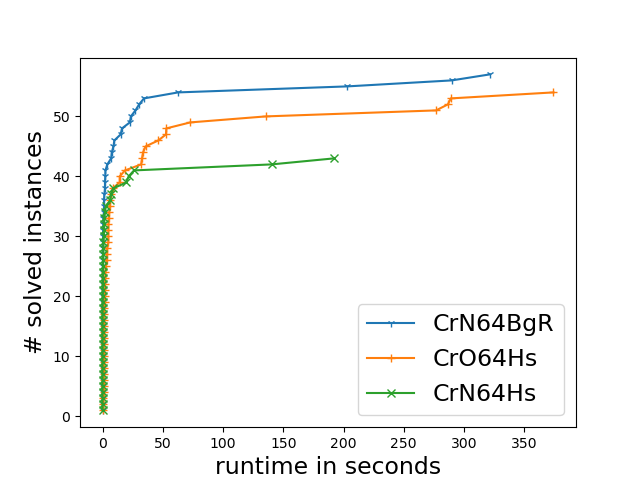
\includegraphics[width=0.5\textwidth]{images/final/old_new}
\end{figure}
Compared to sequential planners PANDA and HyperTensioN, results are mixed.
Looking at PANDA, compared to old CrowdHTN we manage to catch up in domains Hiking Monroe-Fully-Observable and Snake while staying ahead on Blocksworld-HPDDL, Minecraft-Player and Rover-GTOHP. However, overall CrowdHTN still looses out to the more informed PANDA planner. \\
When looking at HyperTensioN, CrowdHTN retains the advantage of high coverage as it's distributed nature makes it less hit-or-miss than HyperTensioN itself. At the same time, improvements in time to plan mean that CrowdHTN almost catches up to HyperTensioN regarding IPC score.

\subsection{Optimizations in CrowdHTN}
\label{eval: crowd optimizations}
In \ref{impl: reduce nodes} we described an improvement to our progression search which let us reduce the number of search nodes we instantiate. To evaluate the impact of this improvement we created an instrumented version of CrowdHTN which let us track this information during planning. We ran this version of CrowdHTN on our benchmark on PC2, using 1 PE, DFS and hash set based loop detection while giving it 300 seconds per instance. We tracked the metadata for all instances, whether a plan was found or not. In addition to the information on actions and world states, we tracked the number of search nodes which were duplicates. The results are shown in table \ref{table: tohtn metadata}. \\
Compared to the other measures, the ratio of tasks which are actions is relatively consistent between domains. It varies from about one third to about two thirds of all tasks. The ratio is lowest for the Logistics-Learned-ECAI-16 domain at $28.2\%$ and highest for Rover-GTOHP at $66.83\%$. \\
When it comes to shared world states, results vary more. On 11 out of the 24 test domains, a world state is on average shared by less than 10 search nodes. This is lowest for the Snake domain with only $1.4$ search nodes per world state. On the other hand for 6 out of our 24 domains more than $1000$ search nodes share one world state, going as far as $\sim3.5 \times 10^8$ search nodes per world state for the Transport domain. \\
To sum these improvements up, our improved search node exploration is a clear benefit on all domains, reducing the number of search nodes we need to represent by at least $28\%$. Sharing world states is more mixed. While sharing is extreme on some domains, it does come at the cost of an additional pointer indirection which may be harmful on domains with little sharing. \\
Regarding loop detection, the results are similarly varied as with state sharing. On 7 out of 24 domains no duplicate nodes were encountered at all and on another 5 domains less than 1\% of nodes were duplicates. At the other end of the spectrum we have Minecraft-Player and Logistics-Learned-ECAI-16 with $\sim30\%$ and Factories-simple with $\sim44\%$ of duplicate nodes. We will return to these numbers in the evaluation of different loop detection techniques in \ref{eval: loop detection}.
\begin{table}[!hbp]
	\caption{Metadata about progression search on our benchmark}
	\label{table: tohtn metadata}
	\centering
	\begin{tabular}{|l|c|r|r|}
		\hline
		Domain & Action\% & Nodes per World State & Loop\% \\
		\hline
		AssemblyHierarchical & 49.71 & 4793.8 & 0.006\\
		Barman-BDI & 33.56 & 10.4 & 4.866\\
		Blocksworld-GTOHP & 50.80 & 6.1 & 0.000\\
		Blocksworld-HPDDL & 49.34 & 83.4 & 1.690\\
		Childsnack & 53.94 & 28800.6 & 0.000\\
		Depots & 45.11 & 7.3 & 2.790\\
		Elevator-Learned-ECAI-16 & 47.89 & 44.9 & 1.663\\
		Entertainment & 49.49 & 7.2 & 0.095\\
		Factories-simple & 31.09 & 2.3 & 43.815\\
		Freecell-Learned-ECAI-16 & 44.42 & 2.5 & 0.000\\
		Hiking & 65.24 & 2.6 & 12.508\\
		Logistics-Learned-ECAI-16 & 28.20 & 4.7 & 30.348\\
		Minecraft-Player & 32.21 & 4.4 & 29.896\\
		Minecraft-Regular & 31.34 & 3.4 & 0.000\\
		Monroe-Fully-Observable & 48.65 & 114.0 & 1.457\\
		Monroe-Partially-Observable & 48.29 & 106.6 & 3.418\\
		Multiarm-Blocksworld & 47.06 & 28.9 & 8.240\\
		Robot & 50.00 & 46207.3 & 0.002\\
		Rover-GTOHP & 66.83 & 3.5 & 0.000\\
		Satellite-GTOHP & 34.66 & 52.5 & 0.013\\
		Snake & 47.16 & 1.4 & 6.948\\
		Towers & 49.99 & 5409.3 & 0.000\\
		Transport & 36.98 & 347788104.5 & 0.000\\
		Woodworking & 49.83 & 21708.8 & 0.442\\
		\hline
	\end{tabular}
\end{table}

\subsection{Search Algorithms}
\label{eval: algorithms}
In section \ref{improv: search algorithms} we presented four search algorithms that we implemented for CrowdHTN. Those algorithms are random DFS, heuristic DFS, A-star like and BFS. We have tested all four algorithms on our test instance set using 4 PEs and a local bloom filter without restarts for loop detection. The results of this test are visualized in figure \ref{figure: eval algorithm}, a summary of coverage and IPC score is presented in table \ref{table: eval algorithm}. \\
Overall, random DFS performed best, followed by heuristic DFS, A-star like search and finally BFS with our best algorithm, random DFS, solving almost twice as many instances and having twice the IPC score of our worst algorithm, BFS. Additionally, we observe a hit-or-miss behavior in both our DFS implementations where plans are either found almost immediately or not at all. Out of the 50 instances solved by random DFS, only 18 were solved in more than 1 and out of these 18 only 9 were solved in more than 10 seconds. BFS on the other hand solves 14 out of 30 instances in more than a second and 11 of these 14 in over 10 seconds. As such, while overall worse performing it does seem to scale better with runtime. \\
Comparing our two DFS-based approaches, we see that random DFS performs better than heuristic DFS guided by our heuristic from section \ref{improv: crowd heuristic}. We attribute this to the fact that we consciously limited our heuristic to information on the hierarchy available from the lifted instance to reduce the time spent on precomputation. Others, such as \cite{holler2020htn} argue that heuristics must utilize both hierarchy and world state information. Our findings corroborate this theory.

\begin{figure}[!hbp]
	\caption{Plotting the number of solved instances per run time for CrowdHTN using DFS, heuristic DFS, A-star like search and BFS}
	\label{figure: eval algorithm}
	\centering
	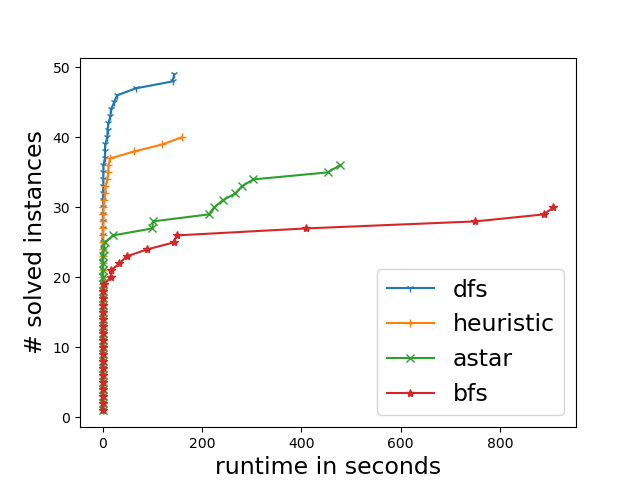
\includegraphics[width=0.5\textwidth]{images/final/search_algorithms.png}
\end{figure}
\begin{table}[!hbp]
	\caption{Coverage and IPC score of our search algorithms using 4 PEs and a local bloom filter}
	\label{table: eval algorithm}
	\centering
	\begin{tabular}{| l | r | r |}
		\hline
		Algorithm 		& Coverage & IPC Score \\
		\hline
		Random DFS 		& 41.7\%	& 43.09 \\ % 50
		Heuristic DFS 	& 33.3\%	& 35.60	\\ % 40
		A-star like 	& 38.3\%	& 27.13 \\ % 36
		BFS 			& 25.0\%	& 21.87	\\ % 30
		\hline
	\end{tabular}
\end{table}

\subsection{Local Loop Detection}
\label{eval: loop detection}
The next feature we tested was the new loop detection based on bloom filters. For our tests we set $k=4$ and limited our false positive probability to $0.001$. The results of this test are shown in figure \ref{figure: eval loop detection}. We see that our bloom filter outperforms the hash set on 32 and 64 PEs, increasing the IPC score by $\sim 5.5$ and coverage by about 6\% when switching from hash set to bloom filter. The gains are so large that 32 PEs using a bloom filter outperform 64 PEs using a hash set. \\
The gains are strongest on the domain Monroe-Fully-Observable and also visible on Snake.
However, we also note that our hash set based loop detection achieves good performance on the Logistics-Learned-ECAI-16 domain while no configuration using bloom filters was able to solve a single instance on this domain. A similar but weaker effect happens in Factories-simple.
Looking at the data in table \ref{table: tohtn metadata} we see that Logistics-Learned-ECAI-16 and Factories-simple are two of the domains with the highest rate of duplicate nodes. We are not sure why Minecraft-Player, the last domain with very high prevalence of duplicate nodes, does not exhibit the same behavior.

\begin{figure}[!hbp]
	\caption{Evaluating CrowdHTN with hash set and bloom filter based loop detection}
	\label{figure: eval loop detection}
	
		\centering
		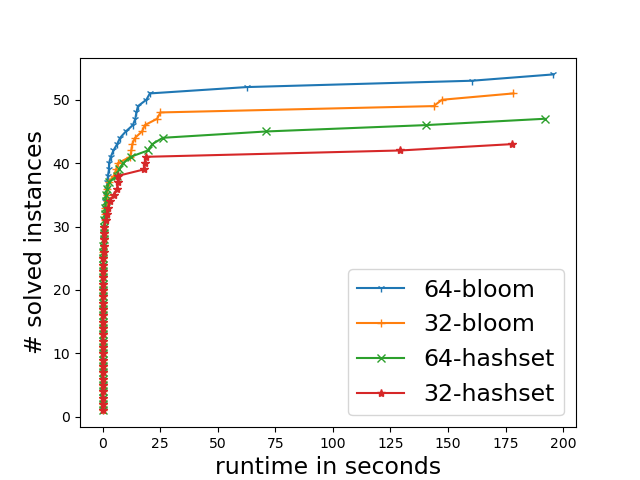
\includegraphics[width=0.5\textwidth]{images/final/loop_detection}
	
	% python3 ../MA_scripts/diagrams.py -files=results_64_dfs_local_bloom_handlepanic_1.csv,results_32_dfs_local_bloom_handlepanic.csv,results_64_dfs_local_hashset_handlepanic.csv,results_32_dfs_local_hashset_handlepanic.csv -names=64-bloom,32-bloom,64-hashset,32-hashset
\end{figure}

\subsection{Probabilistic Restarts and Global Loop Detection}
\label{eval: restarts}
In our next test, we enabled the probabilistic restarts we introduced to guarantee completeness for our bloom filter based loop detection. With runs lasting 900 seconds, we expect $\sum_{t=1}^{899} \frac{1}{t} \approx 7.38$ restarts per run with 5 of these restarts happening within the first 90 seconds. \\
First, we compare CrowdHTN using local bloom filters with and without restarts. The result is shown in figure \ref{figure: restarts}. Overall, probabilistic restarts seem to have a positive effect on coverage and IPC score which is more pronounced on a lower number of PEs. In this way they somewhat mitigate the hit-or-miss nature of our planner. \\
While we see a big difference on 32 PEs, there is little difference on 64 PEs where restarts come with a slight benefit to coverage and a little loss in IPC score. We suspect that, while restarts may increase our chances of finding a plan, they do decrease the chance of finding a plan fast, as they interrupt our search and are especially common right at the beginning. Additionally, there is little difference between restarts on 32 and 64 PEs. We will go further into the specific scaling behavior of CrowdHTN in the benchmark on scalability in \ref{eval: scalability}. \\

\begin{figure}[!hbp]
	\caption{Evaluating CrowdHTN with a local bloom filter with and without restarts}
	\label{figure: restarts}
	\centering
	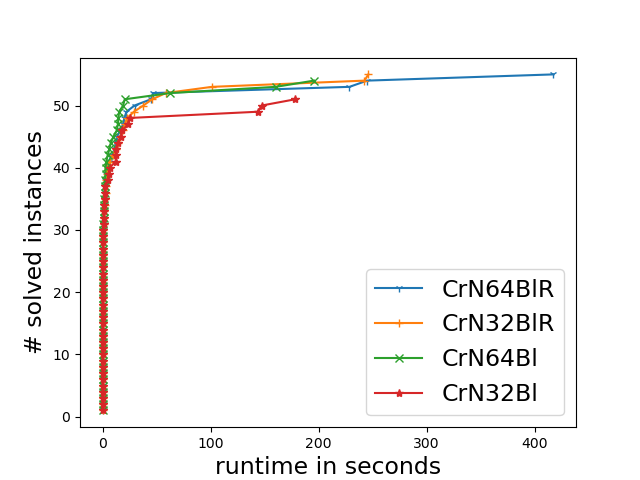
\includegraphics[width=0.5\textwidth]{images/final/restarts}
\end{figure}
\todo{}

\subsection{Global Loop Detection}
\label{eval: global loop}
The last new feature we introduced into CrowdHTN is the ability to perform distributed loop detection and plotted the results in figure \ref{figure: global loops}. Comparing it to CrowdHTN with restarts but no shared information about known search nodes, we get a further small increase in both coverage and IPC score. Among all configurations using bloom filters, CrowdHTN on 64PEs and using global loop detection has the highest coverage and the overall highest IPC score. Similarly, the configuration on 32 PEs is the second best overall, slightly outperforming the 64 PE versions with and without restarts.

\begin{figure}[!hbp]
	\caption{Comparing CrowdHTN with a local bloom filter and restarts with global loop detection}
	\label{figure: global loops}
	\centering
	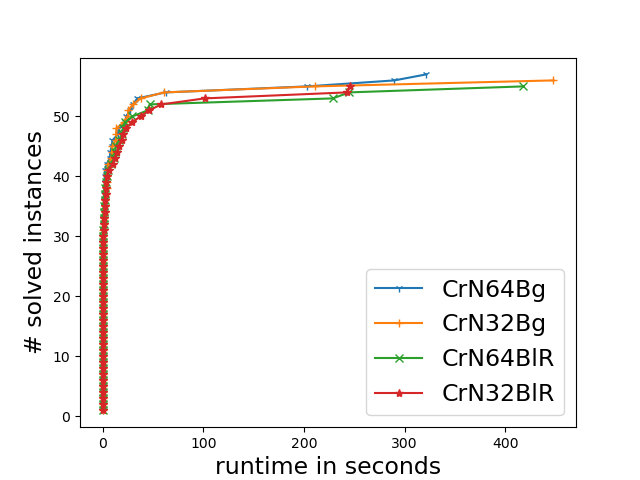
\includegraphics[width=0.5\textwidth]{images/final/global_loops}
\end{figure}

\subsection{Scalability of CrowdHTN}
\label{eval: scalability}
As CrowdHTN is a search-based planner, it has a hit-or-miss characteristic to its performance. This can make it hard to see how its overall performance scales. Many instances are already efficiently solved on a low number of PEs while other instances will remain out of reach even on a high number of PEs. However, over our full benchmark we can still see an increase in overall performance as seen in figure \ref{figure: eval scalability}, even if the effect is relatively weak. \\
To better visualize the scaling behavior of CrowdHTN we will now focus on the Monroe-Fully-Observable domain. It has instances which are somewhat reliably solved for any number of PEs while not being trivial. We ran a separate benchmark of all 20 instances that come with this domain on PC2, testing various configurations of CrowdHTN with local loop detection and no restarts versus global loop detection with restarts. The results are listed in table \ref{table: eval scalability}.\\
Overall we note the clearly increasing IPC score as the number of PEs is increased. Increasing the number of PEs from 4 to 16 has a bigger effect than quadrupling it again to 64. We assume that on this test benchmark the chance of encountering a plan is sufficiently high that we run into diminishing returns as the number of PEs is increased further. Interestingly, CrowdHTN without restarts seems to scale more strongly than CrowdHTN with restarts, as far as the IPC score is concerned. We attribute this to the fact that the IPC score values short run times especially high. Restarts are most frequent during the early phase of planning and may stop CrowdHTN from finding plans very fast. \\
To reduce the impact of randomness, we launched on additional test using instance 11 of the Monroe-Fully-Observable domain. We used CrowdHTN with global loop detection and restarts active, running it 100 times with a time limit of 90 seconds. The distribution of run times is shown in figure \ref{figure: eval scalability box} while success rate and average run times are listed in table \ref{table: eval scalability 2}. All three configurations have high success rate, at 93\%, 97\% and 98\% respectively. The addition of 8 more PEs correlates with an approximately 10 second decrease in average run time. This corresponds to a percentage decrease in run times of 20\% when going from 16 to 24 PEs and of another 30\% when going from 24 to 32 PEs, increases in PEs of 50\% and 33\% respectively.
In reality, gains are even higher as these average run times ignore the cases were the 16 PE configuration failed to find a plan at all.

\begin{figure}[!hbp]
	\caption{Plotting the number of solved instances per run time for CrowdHTN using DFS and a local bloom filter on 64, 16 and 4 PEs}
	\label{figure: eval scalability}
	\centering
	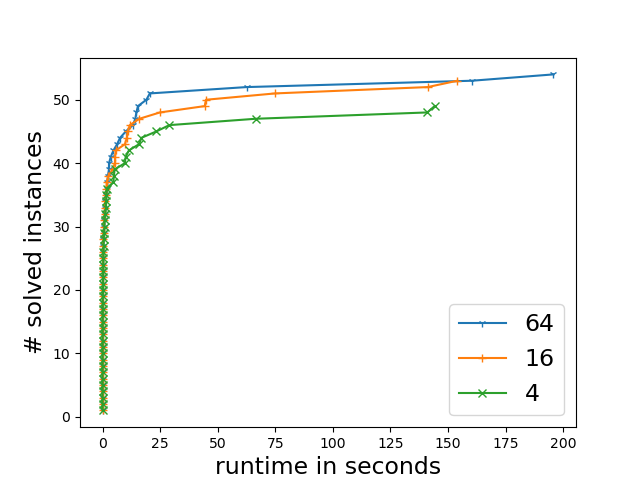
\includegraphics[width=0.5\textwidth]{images/final/scalability}
	% python3 ../MA_scripts/diagrams.py -files=results_64_dfs_local_bloom.csv,results_16_dfs_local_bloom.csv,results_4_dfs_local_bloom.csv  -names=64,16,4
\end{figure}
\begin{table}[!hbp]
	\caption{Evalutating CrowdHTN on 20 instances of the Monroe-Fully-Observable domain}
	\label{table: eval scalability}
	\centering
	\begin{tabular}{|l|rc|rc|rc|rc|rc|rc|}
		\hline
		& \multicolumn{2}{c|}{\textbf{CrN4Bl}} & \multicolumn{2}{c|}{\textbf{CrN16Bl}} & \multicolumn{2}{c|}{\textbf{CrN64Bl}} & \multicolumn{2}{c|}{\textbf{CrN4Bg}} & \multicolumn{2}{c|}{\textbf{CrN16Bg}} & \multicolumn{2}{c|}{\textbf{CrN64Bg}}\\
		& Time & IPC & Time & IPC & Time & IPC & Time & IPC & Time & IPC & Time & IPC\\
		\hline
		01 & 0.2 & 1.00 & 0.1 & 1.00 & 0.4 & 1.00 & 0.1 & 1.00 & 0.7 & 1.00 & 0.1 & 1.00\\
		02 & 161.5 & 0.25 & 30.7 & 0.50 & 1.3 & 0.96 & 115.6 & 0.30 & 10.5 & 0.65 & 22.6 & 0.54\\
		03 & / & 0.00 & 5.7 & 0.74 & 8.4 & 0.69 & 250.5 & 0.19 & 4.0 & 0.80 & 30.5 & 0.50\\
		04 & 0.4 & 1.00 & 0.3 & 1.00 & 0.2 & 1.00 & 0.3 & 1.00 & 0.3 & 1.00 & 0.4 & 1.00\\
		05 & 49.9 & 0.43 & 55.6 & 0.41 & 22.6 & 0.54 & 23.7 & 0.53 & 30.2 & 0.50 & 26.6 & 0.52\\
		06 & 183.9 & 0.23 & 60.1 & 0.40 & 3.5 & 0.82 & 129.0 & 0.29 & 61.7 & 0.39 & 18.2 & 0.57\\
		07 & 18.5 & 0.57 & 7.2 & 0.71 & 3.2 & 0.83 & 5.3 & 0.75 & 2.0 & 0.90 & 4.0 & 0.80\\
		08 & 98.1 & 0.33 & 48.0 & 0.43 & 4.4 & 0.78 & 108.0 & 0.31 & 101.7 & 0.32 & 12.5 & 0.63\\
		09 & 62.3 & 0.39 & 17.7 & 0.58 & 26.0 & 0.52 & 70.8 & 0.37 & 13.5 & 0.62 & 14.3 & 0.61\\
		10 & 122.1 & 0.29 & 33.9 & 0.48 & 23.8 & 0.53 & 80.4 & 0.35 & 61.9 & 0.39 & 11.0 & 0.65\\
		11 & 148.9 & 0.26 & 60.5 & 0.40 & 15.7 & 0.60 & 148.6 & 0.26 & 62.8 & 0.39 & 15.0 & 0.60\\
		12 & 137.5 & 0.28 & 47.9 & 0.43 & 19.4 & 0.56 & 223.4 & 0.20 & 34.7 & 0.48 & 25.6 & 0.52\\
		13 & 19.4 & 0.56 & 2.7 & 0.85 & 1.5 & 0.94 & 7.9 & 0.70 & 0.6 & 1.00 & 1.7 & 0.92\\
		14 & 171.3 & 0.24 & 61.1 & 0.40 & 36.1 & 0.47 & 279.5 & 0.17 & 36.2 & 0.47 & 42.1 & 0.45\\
		15 & / & 0.00 & 6.5 & 0.73 & 4.3 & 0.79 & / & 0.00 & 5.0 & 0.76 & 0.8 & 1.00\\
		16 & / & 0.00 & 6.3 & 0.73 & 2.0 & 0.90 & 7.1 & 0.71 & 6.2 & 0.73 & 4.8 & 0.77\\
		17 & / & 0.00 & 1.6 & 0.93 & 11.2 & 0.64 & / & 0.00 & / & 0.00 & 1.8 & 0.91\\
		18 & 16.7 & 0.59 & 40.0 & 0.46 & 10.3 & 0.66 & 47.2 & 0.43 & 9.0 & 0.68 & 37.7 & 0.47\\
		19 & 1.9 & 0.90 & 5.1 & 0.76 & 1.8 & 0.91 & 15.7 & 0.60 & 15.0 & 0.60 & 5.7 & 0.74\\
		20 & 21.7 & 0.55 & 2.9 & 0.84 & 2.5 & 0.86 & 12.5 & 0.63 & 6.0 & 0.74 & 4.6 & 0.78\\
		\hline
		& & 7.88 & & 12.78 & & 15.01 & & 8.81 & & 12.43 & & 13.98\\
		\hline
	\end{tabular}
\end{table}
\begin{figure}[!hbp]
	\caption{Distribution of run times on Monroe-Fully-Observable instance 11}
	\label{figure: eval scalability box}
	\centering
	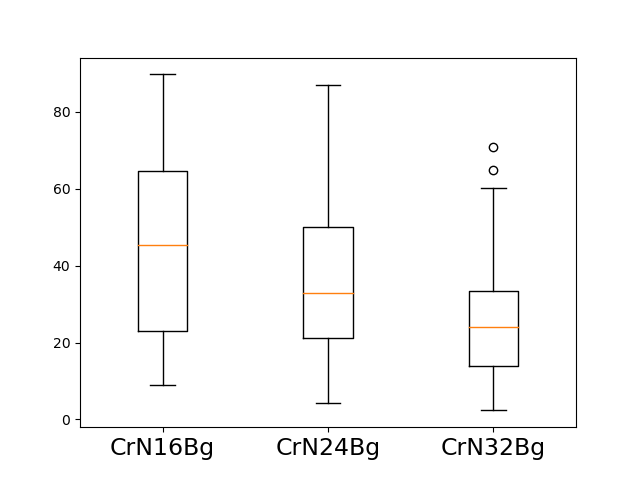
\includegraphics[width=0.5\textwidth]{images/final/scalability_2}
\end{figure}
\begin{table}[!hbp]
	\caption{Success rate and average, minimum and maximum run times of CrowdHTN on Monroe-Fully-Observable instance 11}
	\label{table: eval scalability 2}
	\centering
	\begin{tabular}{|l|c|c|}
		\hline
		Configuration & Success Rate & Average time to plan \\
		\hline
		CrN16Bg 	& 93\% & 45.73  \\
		CrN24Bg		& 97\% & 36.62  \\
		CrN32Bg		& 98\% & 25.98  \\
		\hline
	\end{tabular}
\end{table}

\subsection{Malleable CrowdHTN}
\label{eval: malleable}
To test the behavior of CrowdHTN under malleable conditions, we extended our previous test on scalability. We ran another test on Monroe-Fully-Observable instance 11 using 32 PEs. However, every 20 seconds we injected a second unsolvable job with a time limit of 10 seconds. This means that our normal test oscillates between 32 and 16 PEs every 10 seconds, having an average of 24 PEs available. We compare success rate, average time to plan and the overall distribution of run times with moldable CrowdHTN on 24 PEs. The results are listed in table \ref{table: malleability}. Figure \ref{figure: malleability} shows a box plot of run times per solver. \\
Moldable CrowdHTN on 24 PEs reliably solves this problem in 90 seconds with a success rate of 97\% and an average time to plan of 36.62 seconds. In the ideal case, our malleable CrowdHTN would replicate this behavior. However, we see that malleable CrowdHTN achieves only 69\% success rate with an average time to plan of 31.84 seconds. Looking at the box plot visualizing the distribution of run times, we see that malleable CrowdHTN and moldable CrowdHTN on 24 PEs share the distribution of run times of up to about 50 seconds. Malleable CrowdHTN is missing tail end of the distribution, though, finding no plans beyond the 60 second mark. \\
We suspect that this behavior is due to the way restarts are implemented in CrowdHTN and with how disappearing workers are handled. As we restart with probability $\frac{1}{t}$ at second $t$, we expect about 5 restarts during a 90 second run with 4 of these restarts taking place in the first 30 seconds. Additionally, we handle disappearing PEs by sending the root of their local search space to a random other PE. As in our experiment half of PEs are lost each time another job is introduced, a high number of those messages may be sent to other disappearing PEs, leading to an unexpectedly high loss of information. Restarts seem to mitigate this at the beginning of the search as they are still frequent.
\begin{figure}[!hbp]
	\caption{Distribution of solving times for malleable and moldable CrowdHTN}
	\label{figure: malleability}
	\centering
	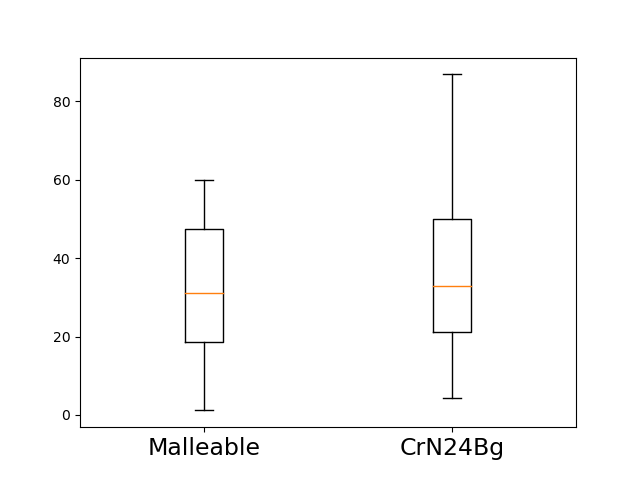
\includegraphics[width=0.5\textwidth]{images/final/malleability}
\end{figure}
\begin{table}[!hbp]
	\caption{Coverage and average run time of malleable and moldable CrowdHTN}
	\label{table: malleability}
	\centering
	
	\begin{tabular}{|l|c|c|}
		\hline
		Configuration & Success rate & Average time to plan \\
		\hline
		Malleable, average 24 PEs	& 69\%	& 31.84 \\
		CrN24Bg						& 97\%  & 36.62 \\
		\hline
	\end{tabular}
\end{table}

\subsection{Discussion}
\label{eval: conclusion}
In this section, we compare our parallel TOHTN planner CrowdHTN as it is integrated into Mallob to the old standalone version of CrowdHTN as well as sequential planners PANDA and HyperTensioN. As shown in the previous sections, the integration of CrowdHTN into Mallob comes with some amount of overhead. We show that CrowdHTN has it's own specific strengths and manages to outperform HyperTensioN in coverage while coming close in overall score. \\
We see the following main results
\begin{itemize}
	\item Our improved node exploration algorithm manages to reduce the number of instantiated nodes from around one to two thirds total.
	\item Bloom filters in loop detection improve both coverage and IPC score overall with the bigger impact on IPC score.
	\item Distributed loop detection and restarts improve coverage and IPC score for smaller numbers of PEs while increasing coverage but potentially decreasing IPC score for a large number of PEs. This may be due to the fact that very fast times to plan are lost in early restarts.
\end{itemize}
Regarding our upgrades to CrowdHTN, we see that the improved node exploration algorithm leads to a big reduction in overall search nodes encountered. Furthermore, bloom filters and distributed loop detection along with restarts both manage to improve the performance of CrowdHTN, with the bigger gain in IPC score coming from the introduction of bloom filters and distributed loop detection with restarts having a bigger impact on overall coverage. \\
In addition to this, we see that overall scaling in CrowdHTN is hard to demonstrate due to the hit-or-miss nature of the planner. However, on well-suited domains such as Monroe-Fully-Observable we demonstrate good scaling behavior of CrowdHTN. \\
Regarding malleability, we see that performance is partially preserved but that loss of information due to frequent reshuffling of a large fraction of PEs can present a problem that the current restarting technique is unequipped to handle.

\begin{table}
	\caption{Domain-wise comparison of sequential planners PANDA, HyperTensioN and parallel planner Crowd in its standalone version}
	\label{table: results old}
	\centering
	\begin{adjustbox}{angle=90}

\begin{tabular}{|l|cc|cc|cc|cc|}
	\hline
	& \multicolumn{2}{c|}{\textbf{PANDA}} & \multicolumn{2}{c|}{\textbf{HyTN}} & \multicolumn{2}{c|}{\textbf{CrO4Hs}} & \multicolumn{2}{c|}{\textbf{CrO64Hs}}\\
	Domain & IPC & Cov & IPC & Cov & IPC & Cov & IPC & Cov\\
	\hline
	AssemblyHierarchical & \textbf{1.0} & 20\%  & \textbf{1.0} & 20\%  & \textbf{1.0} & 20\%  & 0.98 & 20\%  \\
	Barman-BDI & 2.34 & 60\%  & \textbf{4.0} & 80\%  & 1.79 & 40\%  & 1.74 & 40\%  \\
	Blocksworld-GTOHP & \textbf{4.49} & 100\%  & 2.01 & 60\%  & 2.0 & 40\%  & 2.49 & 60\%  \\
	Blocksworld-HPDDL & 1.27 & 40\%  & \textbf{3.98} & 80\%  & 3.21 & 80\%  & 3.01 & 80\%  \\
	Childsnack & 2.64 & 80\%  & \textbf{4.0} & 80\%  & 2.6 & 80\%  & 2.37 & 80\%  \\
	Depots & 3.0 & 60\%  & \textbf{4.0} & 80\%  & 3.63 & 80\%  & 3.6 & 80\%  \\
	Elevator-Learned-ECAI-16 & 3.07 & 100\%  & 3.0 & 60\%  & \textbf{4.06} & 100\%  & 3.86 & 100\%  \\
	Entertainment & \textbf{4.0} & 100\%  & 0.0 & 0\%  & 0.0 & 0\%  & 0.0 & 0\%  \\
	Factories-simple & \textbf{2.0} & 40\%  & 1.0 & 20\%  & 1.91 & 40\%  & 1.86 & 40\%  \\
	Freecell-Learned-ECAI-16 & 0.0 & 0\%  & 0.0 & 0\%  & 0.0 & 0\%  & 0.0 & 0\%  \\
	Hiking & 3.55 & 80\%  & \textbf{4.0} & 80\%  & 2.0 & 40\%  & 1.7 & 60\%  \\
	Logistics-Learned-ECAI-16 & 2.08 & 60\%  & 2.0 & 40\%  & 2.57 & 60\%  & \textbf{2.79} & 80\%  \\
	Minecraft-Player & 0.88 & 40\%  & \textbf{2.0} & 40\%  & 1.73 & 40\%  & 1.62 & 40\%  \\
	Minecraft-Regular & 3.6 & 80\%  & \textbf{4.0} & 80\%  & 3.14 & 80\%  & 2.99 & 80\%  \\
	Monroe-Fully-Observable & \textbf{2.69} & 100\%  & 0.0 & 0\%  & 1.68 & 100\%  & 2.07 & 100\%  \\
	Monroe-Partially-Observable & \textbf{1.53} & 80\%  & 0.0 & 0\%  & 0.93 & 20\%  & 0.82 & 20\%  \\
	Multiarm-Blocksworld & \textbf{1.0} & 20\%  & \textbf{1.0} & 20\%  & \textbf{1.0} & 20\%  & 0.98 & 20\%  \\
	Robot & \textbf{2.0} & 40\%  & \textbf{2.0} & 40\%  & \textbf{2.0} & 40\%  & \textbf{2.0} & 40\%  \\
	Rover-GTOHP & 2.75 & 60\%  & \textbf{4.45} & 100\%  & 3.7 & 100\%  & 3.26 & 80\%  \\
	Satellite-GTOHP & \textbf{3.62} & 100\%  & 0.0 & 0\%  & 0.0 & 0\%  & 0.0 & 0\%  \\
	Snake & 4.45 & 100\%  & \textbf{5.0} & 100\%  & 3.07 & 80\%  & 2.84 & 80\%  \\
	Towers & \textbf{2.6} & 60\%  & 2.0 & 40\%  & 2.2 & 60\%  & 2.15 & 60\%  \\
	Transport & \textbf{2.86} & 80\%  & 1.85 & 40\%  & 0.0 & 0\%  & 0.0 & 0\%  \\
	Woodworking & \textbf{2.0} & 40\%  & 0.35 & 20\%  & 0.0 & 0\%  & 0.0 & 0\%  \\
	\hline
	\textbf{Instances: 120} & 59.4 & 64\% & 51.6 & 45\% & 44.2 & 47\% & 43.1 & 48\% \\
	\hline
\end{tabular}

	\end{adjustbox}
\end{table}

\begin{table}
	\caption{Domain-wise comparison of parallel planner CrowdHTN in various configurations}
	\label{table: results new}
	\centering
	\begin{adjustbox}{angle=90}
		\resizebox{25cm}{!}{
\begin{tabular}{|l|cc|cc|cc|cc|cc|cc|cc|cc|cc|cc|}
	\hline
	& \multicolumn{2}{c|}{\textbf{CrN32Hs}} & \multicolumn{2}{c|}{\textbf{CrN64Hs}} & \multicolumn{2}{c|}{\textbf{CrN4Bl}} & \multicolumn{2}{c|}{\textbf{CrN16Bl}} & \multicolumn{2}{c|}{\textbf{CrN32BL}} & \multicolumn{2}{c|}{\textbf{CrN64Bl}} & \multicolumn{2}{c|}{\textbf{CrN32BlR}} & \multicolumn{2}{c|}{\textbf{CrN64BlR}} & \multicolumn{2}{c|}{\textbf{CrN32Bg}} & \multicolumn{2}{c|}{\textbf{CrN64Bg}}\\
	Domain & IPC & Cov & IPC & Cov & IPC & Cov & IPC & Cov & IPC & Cov & IPC & Cov & IPC & Cov & IPC & Cov & IPC & Cov & IPC & Cov\\
	\hline
	AssemblyHierarchical & 1.0 & 20\%  & 1.0 & 20\%  & 1.0 & 20\%  & 1.0 & 20\%  & 1.0 & 20\%  & 1.0 & 20\%  & 1.0 & 20\%  & 1.0 & 20\%  & 1.0 & 20\%  & \textbf{1.22} & 40\%  \\
	Barman-BDI & 1.0 & 20\%  & 1.97 & 40\%  & \textbf{2.0} & 40\%  & \textbf{2.0} & 40\%  & 1.98 & 40\%  & 1.97 & 40\%  & 1.83 & 40\%  & 1.97 & 40\%  & 1.89 & 40\%  & 1.97 & 40\%  \\
	Blocksworld-GTOHP & 2.0 & 40\%  & 2.0 & 40\%  & 2.0 & 40\%  & 2.0 & 40\%  & 2.0 & 40\%  & 2.39 & 60\%  & 2.32 & 60\%  & 2.2 & 60\%  & \textbf{2.77} & 60\%  & 2.39 & 60\%  \\
	Blocksworld-HPDDL & \textbf{3.05} & 80\%  & 3.0 & 80\%  & 3.03 & 80\%  & 3.02 & 80\%  & 3.0 & 80\%  & 2.98 & 80\%  & 2.82 & 80\%  & 2.88 & 80\%  & 2.88 & 80\%  & 2.83 & 80\%  \\
	Childsnack & 2.86 & 80\%  & 2.83 & 80\%  & \textbf{2.96} & 80\%  & 2.93 & 80\%  & 2.87 & 80\%  & 2.82 & 80\%  & 2.57 & 80\%  & 2.64 & 80\%  & 2.56 & 80\%  & 2.77 & 80\%  \\
	Depots & 3.83 & 80\%  & \textbf{3.95} & 80\%  & 3.92 & 80\%  & 3.86 & 80\%  & 3.86 & 80\%  & 3.85 & 80\%  & 3.77 & 80\%  & 3.82 & 80\%  & 3.79 & 80\%  & 3.87 & 80\%  \\
	Elevator-Learned-ECAI-16 & 4.24 & 100\%  & 4.14 & 100\%  & 4.33 & 100\%  & \textbf{4.36} & 100\%  & 4.31 & 100\%  & 4.29 & 100\%  & 4.02 & 100\%  & 4.11 & 100\%  & 4.1 & 100\%  & 4.22 & 100\%  \\
	Entertainment & 0.0 & 0\%  & 0.0 & 0\%  & 0.0 & 0\%  & 0.0 & 0\%  & 0.0 & 0\%  & 0.0 & 0\%  & 0.0 & 0\%  & 0.0 & 0\%  & 0.0 & 0\%  & 0.0 & 0\%  \\
	Factories-simple & \textbf{2.0} & 40\%  & \textbf{2.0} & 40\%  & 1.0 & 20\%  & 1.0 & 20\%  & 1.0 & 20\%  & 1.0 & 20\%  & 1.0 & 20\%  & 1.0 & 20\%  & 1.0 & 20\%  & 1.0 & 20\%  \\
	Freecell-Learned-ECAI-16 & 0.0 & 0\%  & 0.0 & 0\%  & 0.0 & 0\%  & 0.0 & 0\%  & 0.0 & 0\%  & 0.0 & 0\%  & 0.0 & 0\%  & 0.0 & 0\%  & 0.0 & 0\%  & 0.0 & 0\%  \\
	Hiking & 1.0 & 20\%  & 2.0 & 40\%  & 2.0 & 40\%  & 2.0 & 40\%  & 2.0 & 40\%  & 2.0 & 40\%  & 2.0 & 40\%  & 2.89 & 60\%  & 2.76 & 60\%  & \textbf{3.0} & 60\%  \\
	Logistics-Learned-ECAI-16 & 2.0 & 40\%  & \textbf{3.01} & 80\%  & 0.0 & 0\%  & 0.0 & 0\%  & 0.0 & 0\%  & 0.0 & 0\%  & 0.0 & 0\%  & 0.0 & 0\%  & 0.0 & 0\%  & 0.0 & 0\%  \\
	Minecraft-Player & \textbf{2.0} & 40\%  & \textbf{2.0} & 40\%  & \textbf{2.0} & 40\%  & \textbf{2.0} & 40\%  & \textbf{2.0} & 40\%  & \textbf{2.0} & 40\%  & \textbf{2.0} & 40\%  & \textbf{2.0} & 40\%  & \textbf{2.0} & 40\%  & \textbf{2.0} & 40\%  \\
	Minecraft-Regular & 1.0 & 20\%  & 1.98 & 40\%  & \textbf{3.6} & 80\%  & 3.58 & 80\%  & 3.54 & 80\%  & 3.5 & 80\%  & 3.29 & 80\%  & 3.47 & 80\%  & 3.38 & 80\%  & 3.47 & 80\%  \\
	Monroe-Fully-Observable & 0.72 & 20\%  & 0.0 & 0\%  & 1.92 & 60\%  & 3.3 & 100\%  & 2.69 & 80\%  & \textbf{4.08} & 100\%  & 3.68 & 100\%  & 3.72 & 100\%  & 3.34 & 100\%  & 3.6 & 100\%  \\
	Monroe-Partially-Observable & 0.0 & 0\%  & 0.0 & 0\%  & \textbf{1.0} & 20\%  & 0.0 & 0\%  & \textbf{1.0} & 20\%  & \textbf{1.0} & 20\%  & \textbf{1.0} & 20\%  & \textbf{1.0} & 20\%  & \textbf{1.0} & 20\%  & \textbf{1.0} & 20\%  \\
	Multiarm-Blocksworld & \textbf{1.0} & 20\%  & \textbf{1.0} & 20\%  & 0.0 & 0\%  & \textbf{1.0} & 20\%  & \textbf{1.0} & 20\%  & \textbf{1.0} & 20\%  & 0.99 & 20\%  & \textbf{1.0} & 20\%  & \textbf{1.0} & 20\%  & \textbf{1.0} & 20\%  \\
	Robot & \textbf{2.0} & 40\%  & \textbf{2.0} & 40\%  & \textbf{2.0} & 40\%  & \textbf{2.0} & 40\%  & \textbf{2.0} & 40\%  & \textbf{2.0} & 40\%  & \textbf{2.0} & 40\%  & \textbf{2.0} & 40\%  & \textbf{2.0} & 40\%  & \textbf{2.0} & 40\%  \\
	Rover-GTOHP & 4.43 & 100\%  & 4.4 & 100\%  & \textbf{4.56} & 100\%  & 4.55 & 100\%  & 4.51 & 100\%  & 4.47 & 100\%  & 4.39 & 100\%  & 4.35 & 100\%  & 4.46 & 100\%  & 4.38 & 100\%  \\
	Satellite-GTOHP & 0.0 & 0\%  & 0.0 & 0\%  & 0.0 & 0\%  & \textbf{1.0} & 20\%  & 0.0 & 0\%  & 0.0 & 0\%  & 0.97 & 20\%  & 0.0 & 0\%  & 0.97 & 20\%  & \textbf{1.0} & 20\%  \\
	Snake & 2.0 & 40\%  & 2.0 & 40\%  & 3.1 & 80\%  & 3.89 & 100\%  & 2.85 & 80\%  & 3.4 & 80\%  & 3.94 & 100\%  & 3.98 & 100\%  & 4.02 & 100\%  & \textbf{4.33} & 100\%  \\
	Towers & 2.57 & 60\%  & 2.56 & 60\%  & \textbf{2.66} & 60\%  & 2.65 & 60\%  & 2.62 & 60\%  & 2.61 & 60\%  & 2.61 & 60\%  & 2.56 & 60\%  & 2.52 & 60\%  & 2.6 & 60\%  \\
	Transport & 0.0 & 0\%  & 0.0 & 0\%  & 0.0 & 0\%  & 0.0 & 0\%  & 0.0 & 0\%  & \textbf{1.0} & 20\%  & 0.0 & 0\%  & 0.0 & 0\%  & 0.0 & 0\%  & 0.0 & 0\%  \\
	Woodworking & 0.0 & 0\%  & 0.0 & 0\%  & 0.0 & 0\%  & 0.0 & 0\%  & 0.0 & 0\%  & 0.0 & 0\%  & 0.0 & 0\%  & 0.0 & 0\%  & 0.0 & 0\%  & 0.0 & 0\%  \\
	\hline
	\textbf{Instances: 120} & 38.7 & 36\% & 41.8 & 39\% & 43.1 & 41\% & 46.1 & 44\% & 44.2 & 42\% & 47.4 & 45\% & 46.2 & 46\% & 46.6 & 46\% & 47.4 & 47\% & 48.6 & 48\% \\
	\hline
\end{tabular}
}
\end{adjustbox}
\end{table}